% !TEX root = ../main.tex

\chapter{Data science background} \label{chap:background}

\begin{displayquote}
	\textit{This chapter introduces the general concept of data science and moves the focus of the thesis toward biomedical problems. Relevant examples on how clinical questions can be translated in data science problems are also presented.}
\end{displayquote}

%\section{What is data science and why should we care?} \label{sec:data_science}
% data science vasta: gestione (data engineering) -> data exploration -> machine learning -> data viz
\textit{Data science} is an under development cross-disciplinary field comprising the techniques used to collect and analyze arbitrarily large quantities of measures. The final aim of a data science application is to devise data-driven and statistically sound decision making strategies.
This new field is of extreme interest for both industry and academia. In fact, following the data science philosophy it is possible to obtain highly efficient solutions and new knowledge at the same time and in the same framework.

Nowadays the term data science is becoming ubiquitous; although, deeply understanding what really is and, most importantly, why should we care about it, can be difficult.
This may be due to the confusing fuss that generally surrounds trending terms in the Internet era. Several people, with different backgrounds and different goals, are simultaneously presenting their opinions on the topic\footnote{ And maybe this chapter is just another attempt.} and often their point of view disagree.

Perhaps, focusing on the skills required to be a data scientist may shed some light on the topic. To this regard, in September 2010, Drew Conway published on his popular blog the so-called \textit{Data Science Venn Diagram}, see Figure~\ref{fig:data_science_venn_diagram} \footnote{ Source: \url{https://goo.gl/m4gwmJ}.}.
Let's comment this diagram, separately focusing on each of the three main sets.

\begin{figure}[h!]
	\centering
	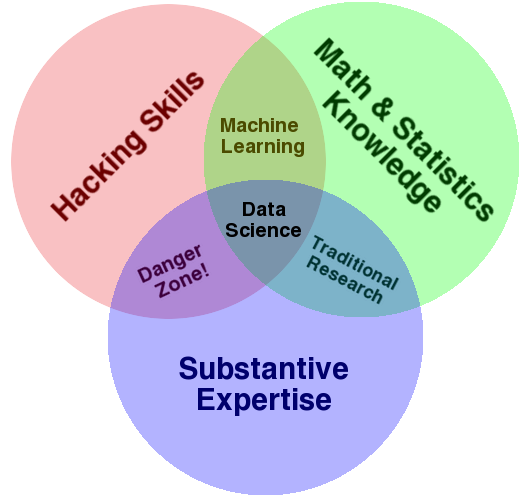
\includegraphics[width=0.8\textwidth]{part1/Data_Science_VD.png}
	\caption{Drew Conway's Data Science Venn Diagram.} \label{fig:data_science_venn_diagram}
\end{figure}

The red set, ironically named \textit{Hacking Skills}, represents all the computer science background that a data scientist need to do his/her job. As shown in the diagram, this  skill is what separates data science from traditional research. In my opinion, this does not mean that traditional researchers are unaware of any computer science skill, but rather that achieving good data science solutions can be, sometimes, a messy task that requires to get hands dirty with several lines of source code.


According to their scope, data collections can have various forms. They may be structured or unstructured, raw or preprocessed, distributed or centralized, and so on. The branch of data science that revolves around developing and maintaining data collections is typically called \textit{data engineering}. Although of great interest, this aspect will not be analyzed in depth in this PhD thesis.

The green set represents the mathematical and statistical background that is needed by data scientists to develop predictive models. Interestingly, Machine Learning (\ac{ML}) lies in the intersection between this set with the red one. We will diffusely discuss about ML in Chapter~\ref{chap:state-of-the-art}, for now we will just think about it as a set of mathematical models and algorithms that, once implemented and deployed on computing facilities, are capable of automatically accomplish complex tasks.

Finally, the blue set, named \textit{Substantive Expertise}, represents the key difference between a data scientist and a classic statistician/data analyst. The main characteristics of data scientists is that they know how to ask the \textit{right} questions to the data. In other words, their domain knowledge allows them to understand which kind of information may be hidden in the data and which data-driven conclusions can be made. Data science produces statistically sound results, in which potentiality and limits of the drawn conclusion are always highlighted. Data scientists shall never \textit{fell in love} with their data, but they should always keep a high level of objectiveness in their analysis. Otherwise, as brilliantly pointed-out by the diagram, we may fear to fall in the intersection between blue and red sets, the \textit{Danger Zone!}


As of today, data are leading recent discoveries in almost every scientific field. In the next sections of this PhD thesis we will focus on the application of data science techniques to biological and biomedical domains.


% DIKW pyramid

%\todo{\begin{itemize}
%\item{Data engineering}
%\item{Data exploration}
%\item{Machine learning and data understanding}
%\item{Data visualization}
%\end{itemize}}



%\section{Challenges in biomedical data science} \label{sec:challenges_biomedical}
% pochi sparsi rumorosi bucati
% this next section needs to be better rewritten
% Scientific progress has always been achieved by systematic observation of natural phenomena followed by experiments, measurements and consequently model formulation.

%
%
% %when dealing with biological studies

\section{Turning biological questions into data science problems} \label{sec:clinical_to_data}
One of the main characteristics of data scientists is being able to devise statistically sound procedures to provide data-driven answers to practical questions. This is very much the case in applied life science studies, where the biological question usually drives the data collection and therefore the data science challenge to be solved.

Although, in order to achieve meaningful results, thorough protocols must be followed, as widely described in Chapter~\ref{chap:state-of-the-art}.
Here, we see an overview of the most recurrent biological questions and their direct translation into data science tasks.

\begin{enumerate}
	
	\item[] \textbf{How to predict phenotypes from observed data?}
	Starting from a collection of input measures that are likely to be related with some known target phenotype, the final goal can be to develop a model that represents the relationship between input and output. Several researches fall in this class, for instance in molecular (\eg lab tests, gene expression, proteomics, sequencing) \cite{angermueller2016deep, okser2014regularized, abraham2013performance} or radiomics/imaging studies (\eg \ac{MRI}, \ac{PET}/\ac{SPECT}, microscopy)~\cite{min2016deep, helmstaedter2013connectomic}. Biological questions of this class are usually tackled by \textit{supervised learning} models. In particular, when the observed clinical outcome is expressed as a one-dimensional continuous value, as in survival analysis, a \textit{single-output regression} problem is posed. Moreover, if the outcome is vector-valued, as in the case of multiple genetic trait prediction~\cite{he2016novel}, the problem can be cast in a \textit{multiple-output regression }framework~\cite{baldassarre2012multi, argyriou2008convex}. Biological studies involving categorical outcomes translate into \textit{classification} problems. In particular, if the clinical outcome assumes only two values, as in the \textit{case}-\textit{control} scenario, the classification problem is said to be \textit{binary}, whilst, if multiple classes are observed, the classification task becomes \textit{multiclass}~\cite{Yuan2016DeepGeneAA, ancona2005regularized} (detailed discussion on this topic is provided in Section~\ref{subsec:supervised_learning}).
	
	\item[] \textbf{Which variables are the most significant?}
	A complementary question revolves around the interpretability of the predictive model. In particular, if dealing with high-dimensional biological data, the main goal can be to identify a relevant subset of meaningful variables for the observed phenomenon. This problem can be cast into a variable/feature selection problem \cite{guyon2002gene}. %To identify a model that uses only a reduced number of variables is of fundamental use in biology as it enhances its interpretability.
	%\todo{group lasso for logistic regression- DNA sequences: \cite{}}
	In particular, a predictive model is said to be \textit{sparse} when it only contains a small number of non-zero parameters, with respect to the number of features that can be measured on the objects this model represents~\cite{hastie2015statistical, meier2008group}. This is closely related to feature selection: if these parameters are weights on the features of the model, then only the features with non-zero weights actually enter the model and can be considered selected (more details on this topic are presented in Section~\ref{subsec:feature_selection}).
	
	\item[] \textbf{How to stratify the data?}
	Collecting measures from several samples, the final goal here is to divide them in homogeneous groups, according to some \textit{similarity} criterion. In data science, this is usually referred to as \textit{clustering}~\cite{hastie2009elements}.
	This happens quite often, for instance when the final goal is to identify the number of groups in some population, or when we look for a single sample which is prototypical of some situation. More details on clustering are presented in Section~\ref{sec:clustering}.
	
	\item[] \textbf{How to represent the samples?}
	In order to formulate a model of some natural phenomenon, it is necessary to design and follow a suitable data collection protocol. A natural question that may arise can be whether the raw collected measures are intrinsically representative of the target phenomenon or if some transformation must be applied in order to achieve a data representation that can be successfully exploited by a predictive model. For instance, it may be plausible to assume that the data lie in a low-dimensional embedding or, conversely, that they can be better represented by a richer polynomial or Gaussian expansion.
	A common solution, in this case, is to take advantage of \textit{feature engineering} techniques to obtain hand crafted features. However, this process can be very time-consuming and it may require the help of domain experts. The process of automatically identifying suitable representations from the data itself is usually referred to as \textit{(un)supervised feature learning}~\cite{angermueller2016deep, mamoshina2016applications} (more details on this topic are provided in Section~\ref{sec:dimred}).
	
	
	\item[] \textbf{Are there recurring patterns in the data?}
	Analyzing data coming from complex domains, one may be interested in understanding whether complex observations can be represented by some combination of simpler events. This typically translates into \textit{adaptive sparse coding} or \textit{dictionary learning} problems~\cite{masecchia2015genome, alexandrov2013signatures}.
	%\todo{add bio example: pathological patterns in tumors from TCGA~\cite{alexandrov2013signatures},
	%Neuroblastoma oncogenesis~\cite{masecchia2015genome}}
	
	
	\item[] \textbf{How to deal with missing values?}
	Applied life science studies must often deal with the issue of missing data. For instance, peaks can be missed in mass-spectrometry~\cite{jung2014adaption} or gene expression levels can be impossible to measure due to insufficient array resolution or image corruption~\cite{stekhoven2011missforest, troyanskaya2001missing}. Common strategies, such as discarding the samples with missing entries, or replacing the holes with mean, median or most represented value, fall short when the missing value rate is high or the number of collected samples is relatively small. This problem usually translates into a \textit{matrix completion} task~\cite{candes2009exact}.
	
\end{enumerate}


